
\chapter{Auswertung} \label{ch:auswertung}

In diesem Kapitel werden MeshGraphNets genutzt, um die Effektivität verschiedener numerischer
Differentialgleichungslöser auf NeuralODEs zu analysieren.
Dafür wird zunächst die \textit{scatter}-Funktion einzeln betrachtet.
Dabei ist besonders die Laufzeitunterschiede zwischen der CPU und GPU Version 
interessant.
Danach werden mehrere Differentialgleichungslöser verwendet, um die NeuralODE 
eines MeshGraphNets auszuwerten.
Die Trainingsdaten und Anfangszustände basieren dabei auf dem von DeepMind 
veröffentlichten \textit{Cylinderflow}-Datensatz für MeshGraphNets\cite{meshgraphnets}.
Diese dienen als Grundlage für das Auswerten der MeshGraphNets und ermöglichen es
den Fehler der verschiedenen Verfahren abzuschätzen.






% 

\chapter{Vergleich des Euler verfahrens mit dem Impliziten Euler verfahren}





\section{Analyse der Scatter Funktion}

In diesem ersten Kapitel wird die \textit{scatter}-Funktion gesondert betrachtet, da
dessen Implementierung entscheidend ist für die impliziten Löser.

Außerdem wurde während der Datenanalyse für dieses Kapitel entdeckt,
dass die Laufzeit der \textit{scatter}-Funktion verbessert werden kann, 
indem die Größe des ziel Arrays beim Funktionsaufruf mit angegeben wird.

Erste Messungen dieser Verbesserung haben eine Zeit Ersparnis von etwa 8 ms bei einer Laufzeit von 21 ms 
versprochen

Genauere Untersuchungen haben jedoch gezeigt, dass dies eine massive Übertreibung war.
Dennoch konnte eine verbesserte Laufzeit erreicht werden, auch wenn diese deutlich geringer ist als zuvor angenommen.

In den folgenden Kapiteln geht es darum, wie es gelungen ist, die Messfehler zu beheben und den Effekt der Verbesserung auf NeuralODEs.


\subsection{Isolierung der \textit{scatter}-Funktion}

Wie bereits angesprochen ist dem der Esten Messung ein Fehler aufgetreten.

Das normale Vorgehen bei der Messung von CUDA Anweisungen ist, 
dass diese synchronisiert werden.
Das heißt, es wird gewartet, bis die asynchrone Anweisung auf der GPU beendet ist.

Das Problem dabei ist das dazu laut der \textit{CUDA}-Dokumentation der Aufruf, mit dem \textit{@sync} Macro aufgerufen werden soll.

Das Problem ist das der \textit{@sync}-Macro nur nach dem auszuführenden Code synchronisiert und nicht davor.

Dies führt dann zu Problemen, wenn vor der zumessenden Aktion eine andere \textit{CUDA}-Operation gestartet wurde.

Auf diese dann ebenfalls gewartet wird. 

Dies verfälscht das Ergebnis, das beobachtet wird und ist der Grund, warum unsere erste Messung so viel längere Laufzeit hatte.

Dies hat es erschwert nachzuweißen, dass es zu dem Gewünschten Laufzeit Verbesserung kommt.

Um Probleme dieser Art zu vermeiden, wurden die folgenden Messungen getrennt von der \textit{NeuralODE} durchgeführt.

Die Größe des \textit{idx}-Arrays wurde für diese Tests nahe an der realen Größe gewählt, um einen Anhaltspunkt für die zeit Ersparnisse zu bekommen.

Alle anderen Werte sind frei erfunden.

So kann es bei dem Index Array zum Beispiel nicht dazu kommen, 
das zwei Einträge denselben wert haben oder die Größe und Form der \textit{src}-Arrays entspricht nicht der Realität.

\begin{table}[h!]
\centering
\begin{tabular}{c|c|c|c|c} 
     GPU & Optimiert & Durchnitt. Laufzeit & Standard Abweichung & Anzahl \\
     \hline
     Ja & Ja     & 452.785 $\mu$s  & 7.278  $\mu$   & 646 * 1000\\
     Ja & Nein   & 496.701 $\mu$s  & 8.920  $\mu$s  &  589 * 1000\\
     Nein & Ja   & 256.064 $\mu$s  & 41.809 $\mu$s  & 1120 * 1000\\
     Nein & Nein & 252.882 $\mu$s  & 36.462 $\mu$s  & 1134 * 1000\\
\end{tabular}
\caption{Messung der \textit{scatter}-Funktion}
\label{table:Scatter}
\end{table}

\begin{table}[h!] 
\centering
\begin{tabular}{c|c|c|c}
     GPU & Durchnitt. Laufzeit & Standard Abweichung & Anzahl \\
     \hline
     Ja     & 39.512 $\mu$s  & 2.835 $\mu$s & 5000 * 1000 \\
     Nein   & 2.628  $\mu$s  &  206.906 ns & 5000 * 1000 \\
\end{tabular}
\caption{Messung der Maximums Berechenung}
\label{table:Maximum}
\end{table}

Die in den Tabellen \ref{table:Scatter} und \ref{table:Maximum} dargestellten Messwerte wurden mit dem \textit{BenchmarkTools.jl} Projekt durchgeführt.

Dabei wurde der Durchschnitt von 1000 Evaluierungen zu einem Messpunkt zusammen gefasst.

Der Grund für diese Maßnahme ist das Speicherreservierungen während der Durchführung der Tests zu einer geringen Menge extrem großer 
Messungen führt.

Dies beeinflusst den Durchschnittswert der Messung nur minimal, hat aber einen sehr großen Einfluss auf dessen Standard Abweichung.

Der durchschnittliche Abstand vom Mittelwert war ursprünglich
um ein Vielfaches größer als der eigentliche Messwert.

Dies führt dazu, dass der Fehler der Messung nicht richtig eingeschätzt werden kann und es demnach nicht sicher ist, ob das gemessene Ergebnis tatsächlich dem entspricht, was erwartet wird.

Es wird angestrebt, diesen Effekt möglichst gering zu halten, da in den NeuralODEs diese Speicher Reservierungen nur einmalig durchgeführt werden müssen.

Es ist anzumerken, das die Anzahl der zusammen gefassten werte ab einem gewissen Werte keinen großen Einfluss auf das Endergebnis mehr hat.
Dies zeigt, dass dies nicht beliebig groß gemacht werden können, bis sich das gewünschte Ergebnis einstellt.

Auf diese Art wurden zwei unterschiedliche Dinge gemessen.

Die Tabelle \ref{Scatter} misst die Laufzeit der gesamten \textit{scatter}-Funktion.
Die Tabelle \ref{Maximum} von Messdaten misst nur die Dauer der Maximumsberechnung, welcher vor allem als Anhaltspunkt für die zu erwartende Unterschiede zwischen den Messungen 
existiert.

Passt die gemessene Verbesserungszeit $R$ nicht zu der erwarteten Zeit der Maximumsberechnung, wäre dies ein Indikator, dass die Laufzeitverbesserung aus einem anderen Grund besser ist oder nicht existiert.

$$
 R_{GPU} = | t_o - t_n | = | 452.785 - 496.701 | = 43.916
$$

$$
 \Delta R_{GPU} = | 1 | \Delta t_o + |-1| \Delta t_n = | 1| * 7.278 +  |-1| * 8.920 = 16.198
$$

Der unterschied zwischen den beiden GPU Messungen ist 43.916 $\mu$s mit einem Fehler von $\pm 16.198 \mu s$.
Da der unterschied zwischen den beiden Werten größer als dessen Fehler ist, kommt es auf der GPU zu einer messbaren Beschleunigung.

Außerdem passt die erwartete Laufzeit Verbesserung von $39,512 \mu s$ zu dem gemessenen Wert unterschied von $43,916 \mu s$.
Da die Werte in der Fehlertoleranz liegen, weißt dies nach, dass das angeben der Zielgröße des \textit{src}-Arrays den gewünschten Effekt hat.

Auf der CPU ergibt sich ein anderes Bild.
$$
R_{CPU} = |t_o - t_n| = | 256.064 \mu s - 252.882 \mu s | =  3.182 \mu s
$$

$$
\Delta R_{CPU} = | 1 | \Delta t_o + |-1| \Delta t_n  = 41.809 \mu s + 36.462 \mu s = 78.271 \mu s
$$


Da die Größe $R_{CPU}$ deutlich geringer ist als dessen absolut Fehler, ist die Messmethode nicht genau genug, um die bessere Laufzeit akkurat zu messen.

Interessant ist die Beobachtung, dass die GPU Variante deutlich langsamer ist als die CPU Variante.

Da dieser Benchmark so geschrieben wurde das die GPU jeden möglichen Vorteil hat.

Dies liegt daran das die Werte im \textit{idx}-Array einzigartig sind.

Das heißt das die \textit{@atomic} aufrufe eigentlich nicht benötigt werden, da nie mehr als zwei Threads in die gleiche speicher Zelle schreiben,
und desshalb auch zu keinen serialisierten \textit{Read-Modify-Write}-Operationen kommt.

Es gibt zwei gründe warum die GPU version dennoch langsammer ist.

Der erst grund ist das es relativ lange dauert daten von der CPU auf die GPU zu kopieren.

Daran lässt sich wenig ändern.

Der zweite Grund ist, dass das hin und her copieren der Daten vom index array in das von der \textit{scatter!}-Funktion verarbeitbares Format, 
lange dauert. Einzelne Messungen haben angedeutet, dass dies etwa 50\% der Laufzeit ausmacht.

....

% Tabelle

Theoretisch könnte direkt auf den übergebenen Daten operiert werden.

Dies ist allerdings nicht besonders leicht und deshalb auch nicht Teil dieser Arbeit.



\subsection{Effekt auf verschiedene Löser Klassen}

In diesem Kapitel wird analysiert, wie sich die Verbesserung der \textit{scatter}-Funktion auf die Laufzeit der unterschiedlichen 
Löser Klassen auswirkt.

Dazu wird exemplarisch der implizite und explizite Euler verwendet.

\begin{table}[h!]
\centering
    \begin{tabular}{c|c|c|c}
         Löser & Optimiert & Sekunden Pro Iteration & Zeit \\
         \hline
         Explicit Euler & Ja & 16.80 ms/it & 0:01:40 \\
         Explicit Euler & Nein & 18.94 ms/it & 0:01:53 \\
         Implicit Euler & Ja & 0.4886 s/it & 7:19:57 \\
         Implicit Euler & Nein &  0.4775 s/it & 17:18:13 \\
    \end{tabular}
    \label{table:langzeitMessung}
    \caption{Messung der NeuralODEs}
\end{table}
In den Daten ist zu beachten, dass die expliziten Methoden aufgrund ihrer kurzen Laufzeit bis zum ende durch gelaufen sind.
Bei den impliziten Lösern wurde aufgrund ihrer langen Berechnungszeit gewartet, bis sich die s/it nicht mehr verändert haben.

Bei den expliziten Lösern ergibt sich ein Unterschied zwischen dem optimierten und langsamen Durchlauf von 2.15 ms/it.

Auf die Gesamtlaufzeit des Problems ergibt sich dadurch eine verbesserte Laufzeit von 15s bzw. 11.5 \%.

Bei den expliziten Lösern ergibt sich ein Unterschied von 0.0111 s/it .
Da die beiden Löser nicht bis zu ende gelaufen sind, muss die Zeit Ersparnisse angenähert werden.

Es ist bekannt, dass nach 17 Stunden etwa 130.000 Schritte durchgeführt wurden und etwa 1/6 der Trajektorie berechnet wurde.

Deshalb kann die Laufzeit Ersparniss $L$ wie folgt approximiert werden.

$$
L = 130.000 \cdot 6 \cdot 0.0111 = 8658s = 144 min = 2.4 Stunden 
$$

Das heißt, es kommt zu einer gesamt Ersparnis von 2.4 Stunden auf eine geschätzte Laufzeit von $17 \cdot 6 $ Stunden.

Dies entspricht einer Verbesserung von 2,4 \%.

Dies zeigt, dass die expliziten Methoden deutlicher mehr von der Verbesserung profitieren.

Der Grund für die geringere Effektivität bei den impliziten Verfahren ist, dass diese mehr Berechnungen durchführen, ohne dafür öfters 
die NeuralODE aufzurufen.

Das Fazit von diesem Kapitel ist, das selbst kleine Verbesserungen in der Laufzeit einen großen Effekt haben können.

Deshalb kann es sich lohnen, nach weiteren kleinen Verbesserungen der Laufzeit zu suchen.





\section{Vergleich des impliziten und expliziten Eulers}

In diesem Kaptiel gehts es darum die auswirkung der Impliciten Löser auf die NeuralODE zu analysieren.

Dazu wurden Drei bespiel trajektorien berechnet.

Welche jeweils mit dem impliziten und expliziten Euler berechnet wurde.

Um beide verfahren möglichst gut miteinander vergleichen zu können wurde darauf geachtet das beide verfahren mit den gleichen einstellungen berechnet wurden.

Dies führt jedoch dazu dass damit die expliziten methoden
überhaupt ihre trajektorie komplett berechenen können, 
die Fehler werte auf einen mindest wert gesetzt werden müssen.

Dies führt dazu das die impliziten methoden ihre eigentlichen stärke ihre schritt weite so anzupassen 
dass diese das bestmögliche ergebniss erreichen nicht 
voll ausnutzen können.

Werden nun die fehler der beiden berechneten trajektorien
direkt miteinander verglichen, kann kaum ein unterschied erkannt werden.

Desshalb wird in der folgenden Graphik
die Differenz der impliziten und expliziten löser geplottet.

$$
d = e_{Implizit} - e_{Explizit}
$$

Dabei wurde explizit auf den Betrag verzichtet damit gesehen werden kann in welchem abschnitt welcher löser den geringeren fehler hat.

Ist also in der Folgenden Graphic die Differenz positiv 
ist der explizite euler besser.

Im Negativen bereich hat dann der impliziten euler den geringeren fehler.

\begin{figure}
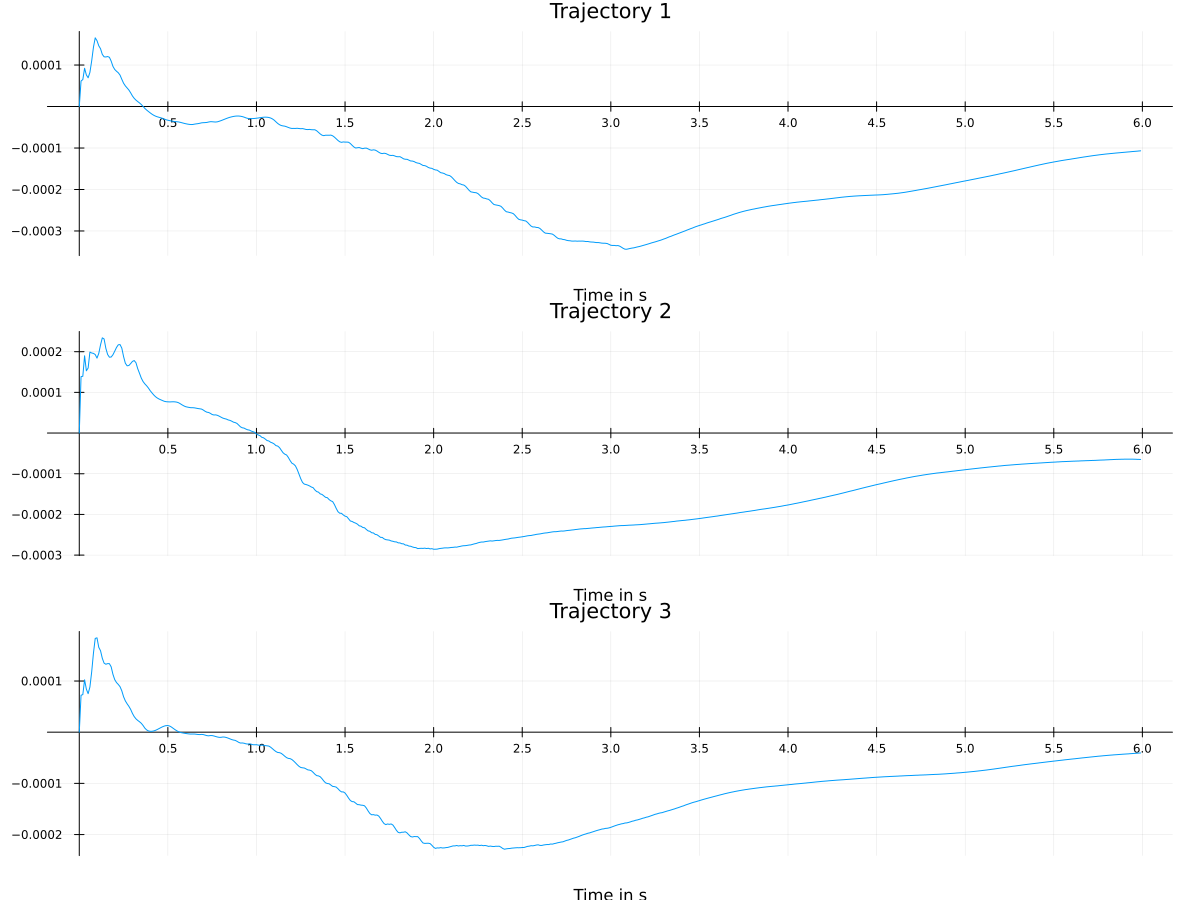
\includegraphics[width=\textwidth]{Data/03_Ergebnisse/errors.png}
\label{fig:eulervergleich}
\end{figure}
In der Graphic kann beobachtet werden, dass beim allen Trajektorien zuerst der Explizite euler das bessere ergebniss liefert.

Dies liegt vorallem daran dass es sich in unserem beispiel 
um einen Flüssigkeits simulation handelt, welche mit einer laminaren strömung begint.

Da diese sich sehr linear verhalten liefert der expliziten 
euler hier sehr gute ergebnisse.

In der Simulation trifft das wasser dann nach 0.5s bis 1s
auf ein objekt.

Dies sorgt für mehr turbulenzen im fluss der flüssigkeit.

Ab diesem Zeitpunkt ist der Implizite euler besser.

Dies liegt vorallem daran das diser mit nicht linearen problemen besser zurecht kommt.

Es fällt aussdem auf das sich beide verfahren mit der zeit
immer weiter annähern.

Dies liegt daran das im allgemeinen mit der zeit die fehler der
trajektorien immer größer werden.

Auch wenn es an hand der daten nicht zeifels frei zu erkennen ist,
lassen die daten vermuten das der impliziten euler auch bei längeren trajektorien ein besseres ergebniss liefert.

Obwohl die daten klar zeigen dass der Implizite Euler bessere
ergebnisse liefert, sollte dieser doch nicht immer gewählt werden.

Wie bereits angesprochen hängt die Qualität der Löser stark vom zu berechnedem problem ab.

Der geringere Fehler der Trajektorie, benötigt jedoch eine deutlich
größere laufzeit.

Bei den expliziten methoden kann einen laufzeit von ein paar minuten 
erwartet werden. Beim impliziten euler kommt es zu einer laufzeit von einigen Tagen. 

In diesem Kaptiel wurden die Vor- und Nachteil der beiden Methoden vorgestellt.

Wie diese Zwei verfahren miteinander verbunden werden können geht es im nächsten Kapitel.









\section{Automatischer Löser Wechsel}

Im Kaptiel \ref{} wurde die Vor- und Nachteile der Impliziten und expliziten Differenzialgelichungslöser 
vorgestellt.

In diesem Kapitel wird untersuch wie die vorteile beider verfaheren so miteinander verbunden 
werden können, dass das projekt so wohl mit einer hohen genauichkeit, als auch einer verträglichen laufzeit
ausgeführt werden kann.
Wie bereits gezeigt wurde, liefern die unterschiedlichen löser zu unterschiedlichen zeitpunkten
unterschiedlich gute ergebnisse.
Das \textit{DifferentialEquations.jl} Projekt bietet dafür die möglichkeit automatisch 
zwischen verschiedenen lösungsverfahren zuwechseln.

Dies geschieht meist abhängig von aktuellen Fehler, es können aber auch eigene Kriterien entwickelt werden.

Dabei ist jedoch zu beachten das dies nicht mit allen Verfahren möglich ist.

So ist es zum beispiel nicht möglich den impliziten mit dem expliziten euler zu verbinden.

Deshalb wird im folgendem der \textit{Tsit5} mit dem \textit{Rosenbrock23} verbunden. Dieser Algorithmus wird im folgendem als AutoTsit5 bezeichnet.

Dessenlaufzeit kann stark varieren. Je nach problem kann die laufzeit zwischen ein paar sekunden und
ein paar studen sein.

In den für dieses Kaptiel berechneten trajectorien, war die geringste laufzeit 19s und die längste 2h.

Die genaue laufzeit hängt sehr stark von den benötigten fehler toleranzen und der problem größe ab.

Im folgenden wird das bereits genannte verfahren mit dem expliziten euler verglichen.

\begin{figure}[h]
    \centering
    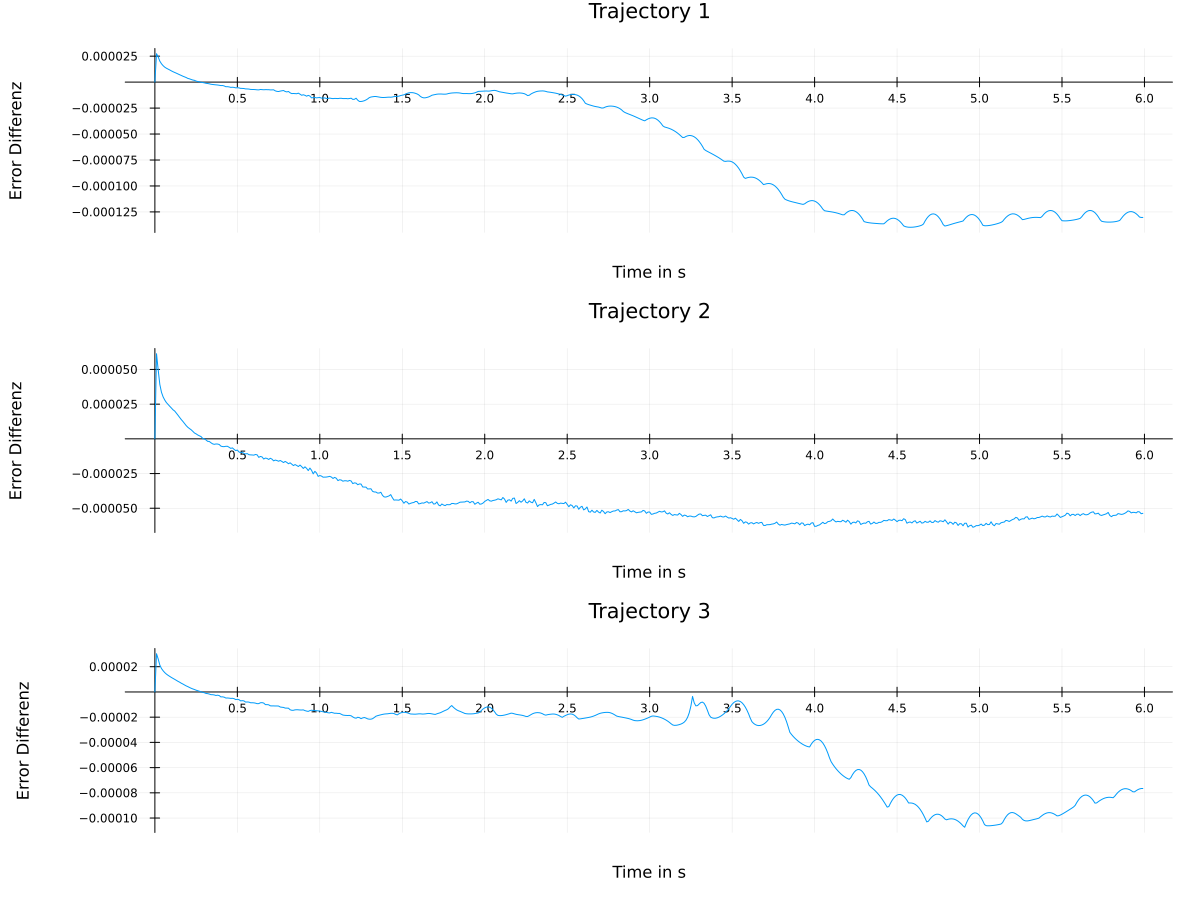
\includegraphics[width=\textwidth]{Data/03_Ergebnisse/autoswitching/errors_explizit_composit.png}
    \caption{Vergleich mit Explizit Algorithm}
    \label{fig:vergleichexplizit}
\end{figure}

In der Grafik \ref{fig:vergleichexplizit} wird die differenz zwischen dem Expliziten Euler und dem AutoTsit5 verglichen.

In den ersten 0.5 sekunden ist die differenz positiv, dies bedeutet, dass
der Explizite euler bessert.

Danach liefert der AutoTsit dann ein konstant besseres ergebniss.




\begin{figure}[h]
    \centering
    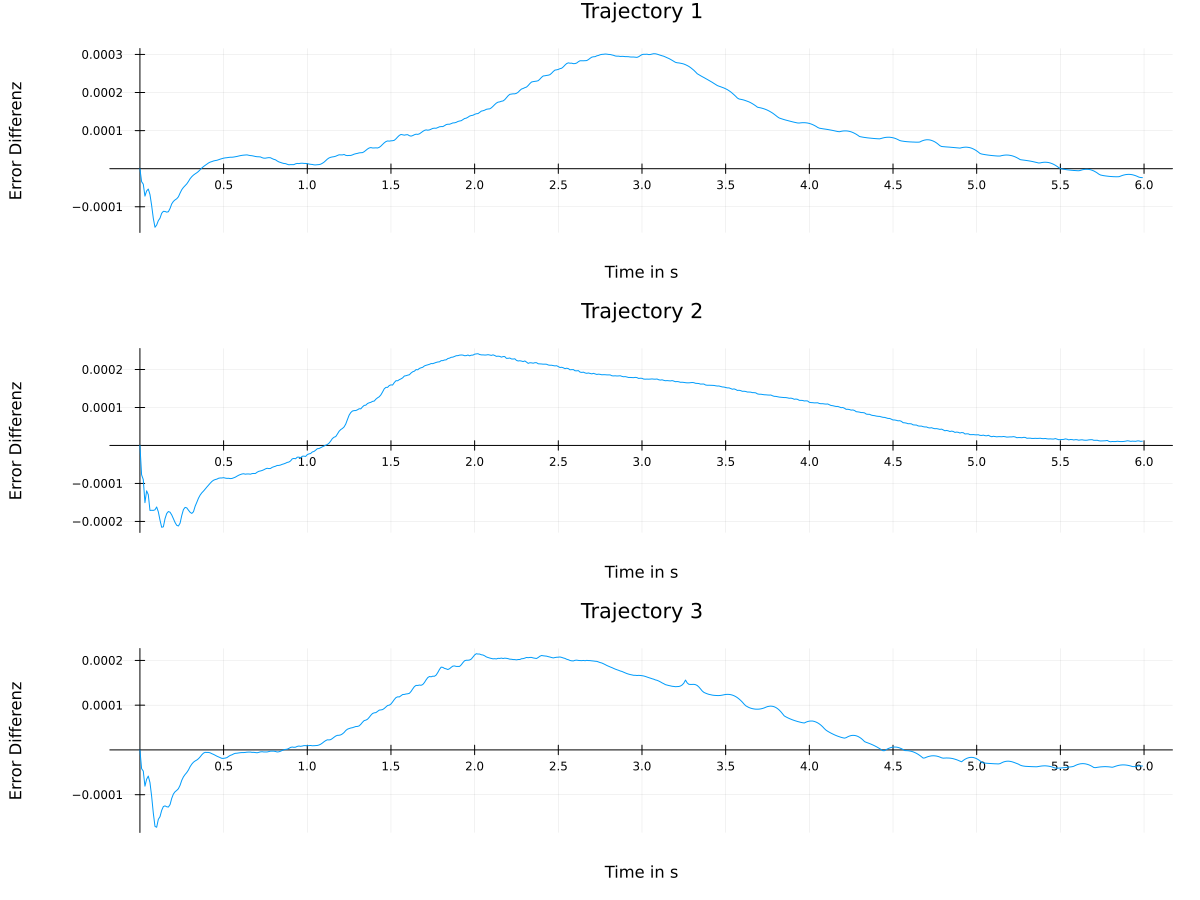
\includegraphics[width=\textwidth]{Data/03_Ergebnisse/autoswitching/errors_implizit_composit.png}
    \caption{Vergleich mit Implizit Algorithm}
    \label{fig:vergleichimplizit}
\end{figure}

In der Graphik \ref{fig:vergleichimplizit} wird beobachtet,
dass der AutoTsit5 am Anfang einbessers ergebniss liefert.

Nach etwa 1 sekunde wird dann der Implizite Euler besser.

Besonders ist vorallem das der Unterschiede zwischen beiden verfahren gegen ende sich sehr stark null annähert und bei zwei der drei trajektorien gegen ende wieder ein bessers ergebniss liefert.

Dies lässt vermuten das der AutoTsit bei längeren trajektorien, ein sehr gutes ergebniss liefert.












\section{Funktionierende Löser}

In diesem Abschnitt wird ein überblick darüber gegeben, welche 
ODE Löser nach dem hinzufügern der in \ref{} Vorgestellten 
version der \textit{scatter}-Funktion nun möglich sind.

Wichtig ist dabei das es nicht möglich ist jeden löser ausführlich zu testen
da diese zum Teil eine sehr lange laufzeit haben.

Aufgrund dessen wurde jeder der im folgenden grafik als Funktionend 
bezeichnet solange laufen gelassen bis dieser den ersten zeit schritt gemacht hat.

Der Grund für diese vorgehens weiße ist dass die löser an diesem punkt meistens scheitern.

Wenn dieser punkt überschritten war dann kam es erfahrungs gemäß zu keinen 
weitern problem eine 100\%-tige garantie lieftert dies aber nicht.

\begin{table}[]
    \centering

    \begin{tabular}{p{5cm}|c|p{5cm}}
        Name & Funktionale & Fehler \\
        \hline\hline
        ImplicitEuler & true & \\ 
ImplicitMidpoint & true & \\ 
Trapezoid & true & \\ 
TRBDF2 & true & \\ 
SDIRK2 & true & \\ 
Kvaerno3 & true & \\ 
KenCarp3 & true & \\ 
Cash4 & true & \\ 
Hairer4 & true & \\ 
Hairer42 & true & \\ 
Kvaerno4 & true & \\ 
KenCarp4 & true & \\ 
KenCarp47 & true & \\ 
Kvaerno5 & true & \\ 
KenCarp5 & true & \\ 
KenCarp58 & true & \\ 
RadauIIA3 & false & Error: DimensionMismatch: arguments must have the same number of rows \\
RadauIIA5 & false & Error: DimensionMismatch: arguments must have the same number of rows \\
PDIRK44 & false & Error: `@threads :static` cannot be used concurrently or nested \\
ROS3P & true & \\ 
Rodas3 & true & \\ 
RosShamp4 & true & \\ 
Veldd4 & true & \\ 
Velds4 & true & \\ 
GRK4T & true & \\ 
GRK4A & true & \\ 
Ros4LStab & true & \\ 
Rodas4 & true & \\ 
Rodas42 & true & \\ 
Rodas4P & true & \\ 
Rodas4P2 & true & \\ 
Rodas5 & true & \\ 
Rodas5P & true & \\ 
Rosenbrock23 & true & \\ 
Rosenbrock32 & true & \\ 
RosenbrockW6S4OS & true & \\ 
ROS34PW1a & true & \\ 
ROS34PW1b & true & \\ 
ROS34PW2 & true & \\ 
ROS34PW3 & true & \\ 
ImplicitEulerExtrapolation & true & \\ 
ImplicitEulerBarycentricExtrapolation & true & \\ 
ImplicitDeuflhardExtrapolation & true & \\ 
ImplicitHairerWannerExtrapolation & true & \\ 
PDIRK44 & false & Error: `@threads :static` cannot be used concurrently or nested \\
LawsonEuler & false & Error: ArgumeError: Caching can only be used with SplitFunction \\
NorsettEuler & false & Error: ArgumeError: Caching can only be used with SplitFunction \\
ETD2 & false & Error: type ODEFunction has no field f1 \\
ETDRK2 & false & Error: ArgumeError: Caching can only be used with SplitFunction \\
ETDRK3 & false & Error: ArgumeError: Caching can only be used with SplitFunction \\
ETDRK4 & false & Error: ArgumeError: Caching can only be used with SplitFunction \\
HochOst4 & false & Error: ArgumeError: Caching can only be used with SplitFunction \\
Exprb32 & false & Error: DimensionMismatch: array could not be broadcast to match destination \\
Exprb43 & false & Error: DimensionMismatch: A has dimensions (3792,3792) but B has dimensions (2,1896) \\
Exp4 & false & Error: AssertiError: Dimension mismatch \\
EPIRK4s3A & false & Error: AssertiError: Dimension mismatch \\
EPIRK4s3B & false & Error: AssertiError: Dimension mismatch \\
EPIRK5P1 & false & Error: AssertiError: Dimension mismatch \\
EPIRK5P2 & false & Error: AssertiError: Dimension mismatch \\
EPIRK5s3 & false & Error: DimensionMismatch: tried to assign 2×1896 array to 3792×1 destination \\
EXPRB53s3 & false & Error: AssertiError: Dimension mismatch \\
SSPSDIRK2 & false & Error: MethError: Cannot `convert` an object of type Float32 to an object of type CUDA.CuArray{Float32, 2, CUDA.Mem.DeviceBuffer} \\
    \end{tabular}
    \caption{Caption}
    \label{tab:my_label}
\end{table}



\section{Zusammenfassung}
